\RequirePackage{luatex85}
\documentclass{standalone}

% Default preamble
\usepackage{tikz}
\usepackage{pgfplots}
\pgfplotsset{compat=newest}
\usepgfplotslibrary{groupplots}
\usepgfplotslibrary{polar}
\usepgfplotslibrary{smithchart}
\usepgfplotslibrary{statistics}
\usepgfplotslibrary{dateplot}
\usepgfplotslibrary{ternary}

% Custom preamble from global variable:
\usetikzlibrary{patterns}
\usepackage{xcolor}
\definecolor{cred}{HTML}{ED1C24}
\definecolor{cgrey}{HTML}{7F7F7F}
\definecolor{cblue}{HTML}{00A2E8}
\definecolor{cgreen}{HTML}{22B14C}
\definecolor{cyellow}{HTML}{FFF200}
\definecolor{corange}{HTML}{EA7904}
\definecolor{cpurple}{HTML}{9100FC}
\definecolor{julia1}{HTML}{1F77B4}
\definecolor{julia2}{HTML}{FF7F0E}
\definecolor{julia3}{HTML}{2CA02C}
\definecolor{julia4}{HTML}{D62728}

\usepackage{caption}
\usepackage{subcaption}
\usepackage{amsmath}

% borrowed from <https://tex.stackexchange.com/a/145967/95441>
\pgfmathdeclarefunction{fpumod}{2}{%
    \pgfmathfloatdivide{#1}{#2}%
    \pgfmathfloatint{\pgfmathresult}%
    \pgfmathfloatmultiply{\pgfmathresult}{#2}%
    \pgfmathfloatsubtract{#1}{\pgfmathresult}%
    % replaced `0' by `5' to make it work for this problem
    \pgfmathfloatifapproxequalrel{\pgfmathresult}{#2}{\def\pgfmathresult{5}}{}%
}
\pgfplotsset{boxplot legend/.style={
    legend image code/.code={
        \draw[#1,fill=cblue,thin] (0cm,-0.1cm) rectangle (0.4cm,0.1cm)
        (0.2cm,-0.1cm) -- (0.2cm,-0.2cm) (0.05cm,-0.2cm) -- (0.35cm,-0.2cm)
        (0.2cm,0.1cm) -- (0.2cm,0.2cm) (0.05cm,0.2cm) -- (0.35cm,0.2cm);
     \path (0cm,0.24cm) (0cm,-0.24cm);  
    },
}}

\renewcommand{\familydefault}{\sfdefault}

% Run boxplot-hepg2.jl interactively
% Median: hepg2_median
% Lower quartile: hepg2_lq
% Upper quartile: hepg2_uq
% Lower whisker: hepg2_lw
% Upper whisker: hepg2_uw
% Whiskers (combined): hepg2_whiskers

\begin{document}

    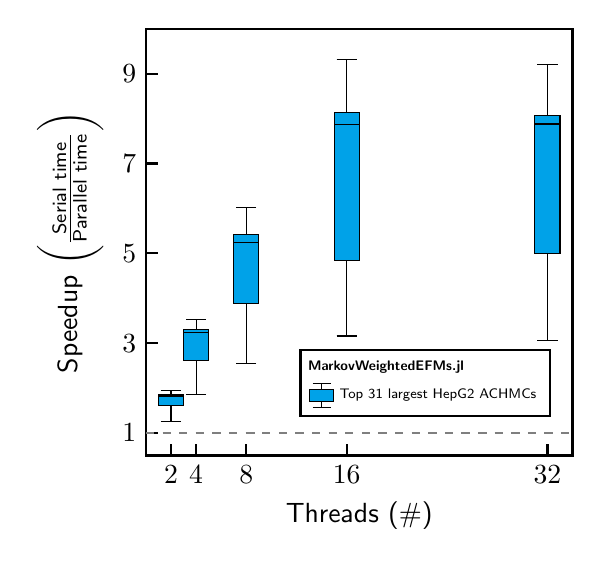
\begin{tikzpicture}
        \begin{axis}[%
            height=7cm,
            width=7cm,
            boxplot/draw direction=y,
            xlabel = Threads (\#),
            ylabel = Speedup $\bigg(\frac{\text{Serial time}}{\text{Parallel time}}\bigg)$,
            legend cell align = {left},
            xmajorgrids={false},
            ymajorgrids={false},
            xtick pos = bottom,
            ytick pos = left,
            legend style={%
                font=\tiny,
                thick,
                at={(0.95,0.25)},
            },
            legend entries={\hspace*{-0.4cm}\textbf{MarkovWeightedEFMs.jl}, Top 31 largest HepG2 ACHMCs},
            legend image post style={scale=0.75},
            axis line style={thick,black},
            minor tick style={draw=none},
            xtick style={/pgfplots/on layer=axis foreground, thick, black},
            ytick style={/pgfplots/on layer=axis foreground, thick, black},
            xmin={0},
            xmax={34},
            xtick={2,4,8,16,32},
            ymin={0.5},
            ymax={10},
            ytick={1, 3, 5, 7, 9}
        ]
            \addlegendimage{empty legend}
            \addplot[%
                forget plot,
                fill=cblue,
                boxplot prepared={%
                    draw position = -2,
                    lower whisker = 1,
                    lower quartile= 1,
                    median        = 1,
                    upper quartile= 1,
                    upper whisker = 1,
                    box extend    = 2.0
                },
            ] coordinates {};
            \addplot[%
                forget plot,
                fill=cblue,
                boxplot prepared={%
                    draw position = 2,
                    lower whisker = 1.2630051130912274,
                    lower quartile= 1.6032135513668697,
                    median        = 1.8229211001873333,
                    upper quartile= 1.8520566777519614,
                    upper whisker = 1.9355235227925298,
                    box extend    = 2.0
                },
            ] coordinates {};
            \addplot[%
                forget plot,
                fill=cblue,
                boxplot prepared={%
                    draw position = 4,
                    lower whisker = 1.8647520808195945,
                    lower quartile= 2.6147046495313653,
                    median        = 3.2284909036836495,
                    upper quartile= 3.3033840165641823,
                    upper whisker = 3.5173504009386516,
                    box extend    = 2.0
                },
            ] coordinates {};
            \addplot[%
                forget plot,
                fill=cblue,
                boxplot prepared={%
                    draw position = 8,
                    lower whisker = 2.538328408806043,
                    lower quartile= 3.892301524291141,
                    median        = 5.244514549507511,
                    upper quartile= 5.417714406509516,
                    upper whisker = 6.0264821338803305,
                    box extend    = 2.0
                },
            ] coordinates {};
            \addplot[%
                forget plot,
                fill=cblue,
                boxplot prepared={%
                    draw position = 16,
                    lower whisker = 3.160087879688405,
                    lower quartile= 4.830446139081701,
                    median        = 7.860591564725095,
                    upper quartile= 8.139196454110749,
                    upper whisker = 9.32177982819481,
                    box extend    = 2.0
                },
            ] coordinates {};
            \addplot[%
                forget plot,
                no marks,
                fill=cblue,
                boxplot prepared={%
                    draw position = 32,
                    lower whisker = 3.0622144015104995,
                    lower quartile= 4.98753722900201,
                    median        = 7.87888796200494,
                    upper quartile= 8.062076310409761,
                    upper whisker = 9.206538313729814,
                    box extend    = 2.0
                },
            ] coordinates {};

            \addlegendimage{boxplot legend, black}
            \addplot[forget plot,samples=2, smooth,domain=1:1,cgrey,dashed] coordinates {(0,1)(34,1)};
        \end{axis}
    \end{tikzpicture}

\end{document}

